\section{Kinematic coverage and binning}

\begin{wrapfigure}{r}{0.35\textwidth}
	\vspace*{-2em}
	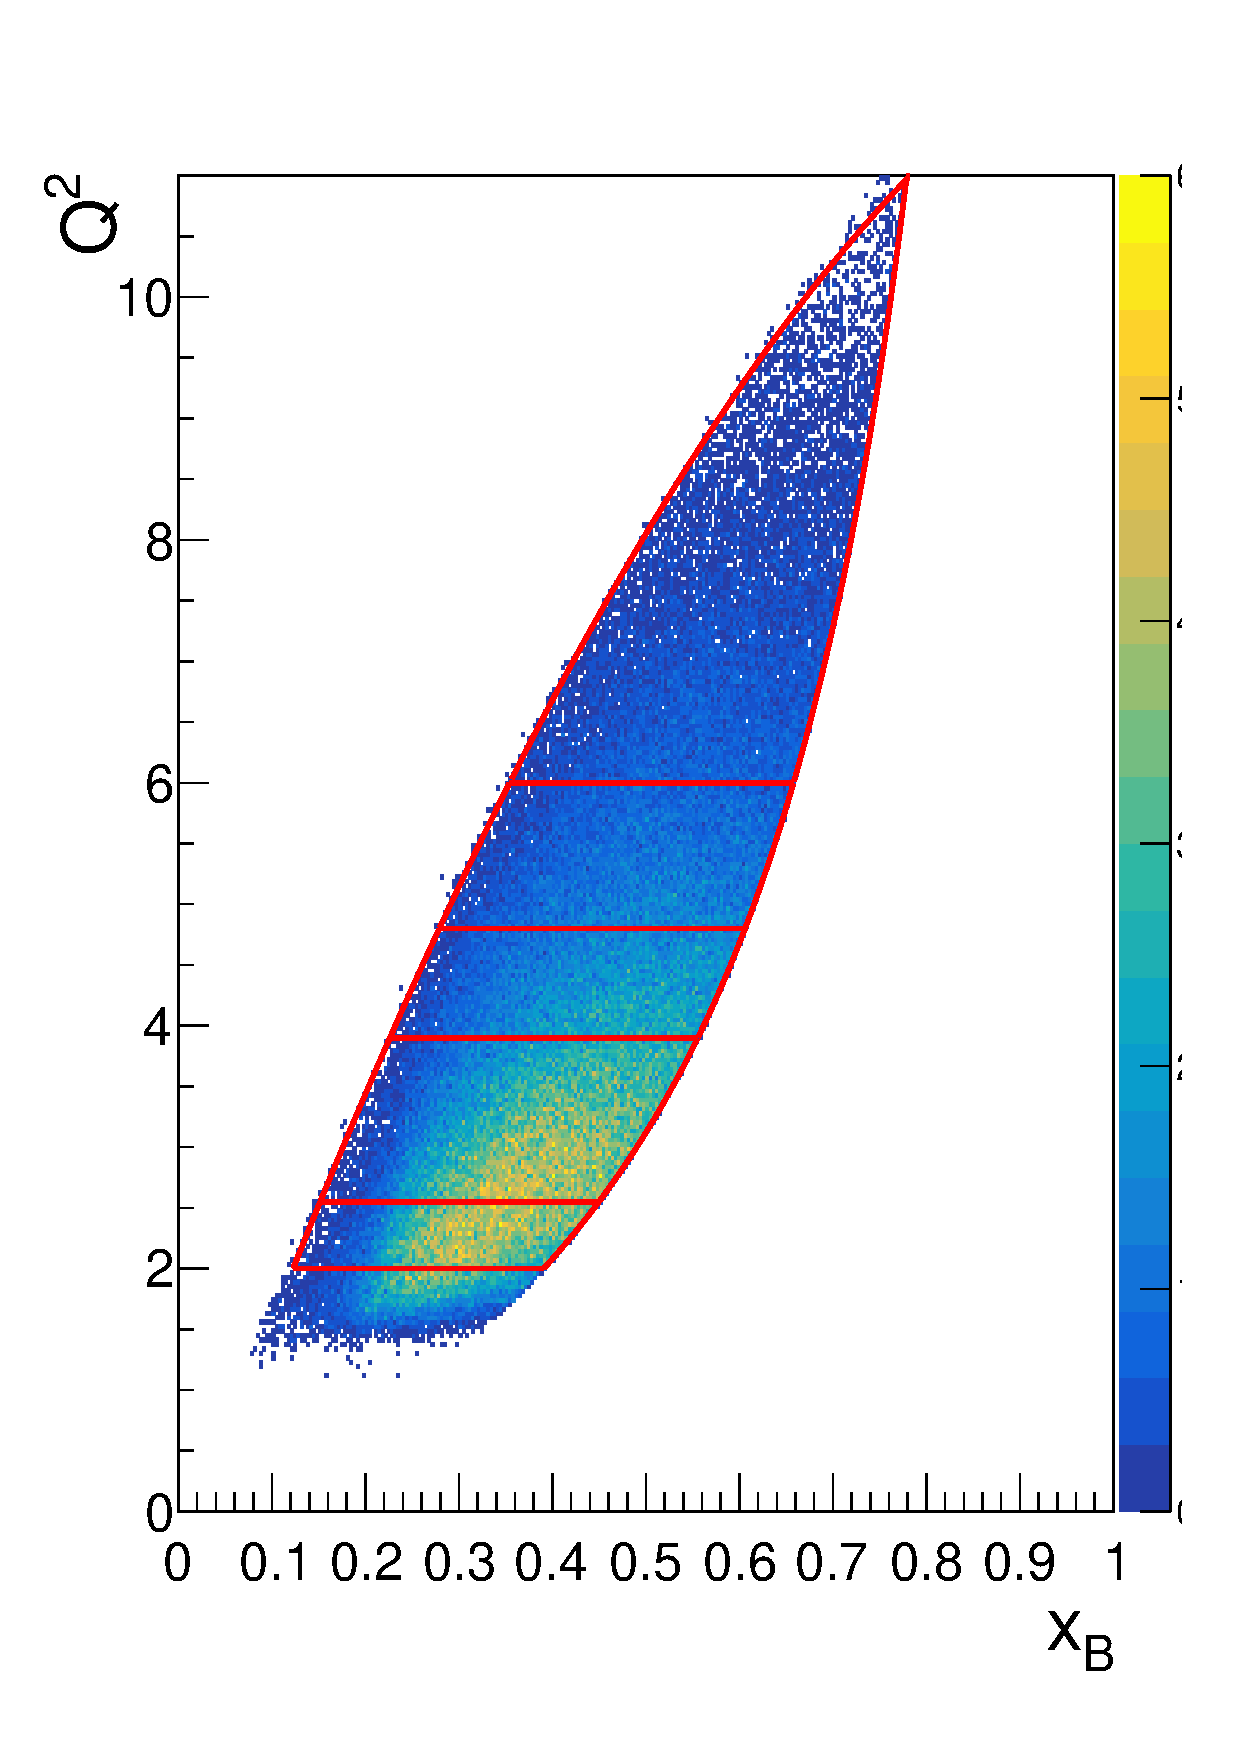
\includegraphics[page=1,width=0.97\linewidth]{figures/eppi0.inb.root.bins.pdf}
	\caption{$Q^2$ vs $x_B$ for $ep\rightarrow ep\pi^0$ events. Red lines show $Q^2$ vs $x_B$ kinematic bins for inbending dataset.}
	\label{fig:Q2vsxb}
\end{wrapfigure}

The $Q^2$ vs $x_B$ 2D distribution is shown on Fig.~\ref{fig:Q2vsxb} for exclusive $ep\rightarrow ep\pi^0$ events.
5 $Q^2$ vs $x_B$ bins are chosen to have two lowest $Q^2$ bins with kinematic values similar to CLAS6 data.
Each of $\{Q^2,x_B\}$ bin was split into 3 $-t$ bins, and each of 3D $\{Q^2,x_B,-t\}$ bins was split into 9 equidistant  $\phi$ bins.

\begin{itemize}
	\item $2<Q^2<2.56$ GeV
	\begin{itemize}
		\item 3 $\left<-t\right>$ bins: $[0, 0.39], [0.39, 0.71], [0.71, 2]$~GeV$^2$
	\end{itemize}
	\item $2.56<Q^2<3.8$ GeV
	\begin{itemize}
		\item 3 $\left<-t\right>$ bins: $[0, 0.47], [0.47, 0.87], [0.87, 2]$~GeV$^2$
	\end{itemize}
	\item $3.8<Q^2<4.8$ GeV
	\begin{itemize}
		\item 3 $\left<-t\right>$ bins: $[0, 0.57], [0.57, 0.99], [0.99, 2]$~GeV$^2$
	\end{itemize}
	\item $4.8<Q^2<6$ GeV
	\begin{itemize}
		\item 3 $\left<-t\right>$ bins: $[0, 0.67], [0.67, 1.09], [1.09, 2]$~GeV$^2$
	\end{itemize}
	\item $6<Q^2<11$ GeV
	\begin{itemize}
		\item 3 $\left<-t\right>$ bins: $[0, 0.91], [0.91, 1.37], [1.37, 2]$~GeV$^2$
	\end{itemize}
\end{itemize}

5 2D distributions of $-t$ vs $\phi$ for each of $\{Q^2,x_B\}$ bins are shown on Fig.~\ref{fig:tphibins}.


\begin{figure}[hbt]
	\centering
	\includegraphics[page=21,width=0.32\linewidth]{figures/eppi0.inb.root.bsa.pdf}
	\includegraphics[page=22,width=0.32\linewidth]{figures/eppi0.inb.root.bsa.pdf}
	\includegraphics[page=23,width=0.32\linewidth]{figures/eppi0.inb.root.bsa.pdf}

	\includegraphics[page=24,width=0.32\linewidth]{figures/eppi0.inb.root.bsa.pdf}
	\includegraphics[page=25,width=0.32\linewidth]{figures/eppi0.inb.root.bsa.pdf}

	\caption{The distribution for $-t$ vs $\phi$ for 5 $\{Q^2,x_B\}$ bins of inbending dataset.}.
	\label{fig:tphibins}
\end{figure}


\section{Beam Spin Asymmetry}

\begin{equation}
	BSA=\frac{1}{P_b}\frac{n^+-n^-}{n^++n^-}
\end{equation}
where $P_b$ is average beam polarization, $n^{+(-)}$ is the number of exclusive events in each 4D $\{Q^2,x_B,-t,\phi\}$ bin with sideband background subtracted.

\subsection{Sideband background subtraction}

Exclusivity cuts provide a very effective way to clean the data sample but a fraction of background events still pass all exclusivity cuts and needs to be taken into account.
These events are clearly visible on the plot of invariant mass of two photons as a linear background underneath gaussian peak, as shown on Fig.~\ref{fig:mgginq2xbtt}.
The number of events are counted in $[-5\sigma,-3\sigma]$ and $[3\sigma,5\sigma]$ regions and multiplied by 1.5 to estimate the number of events underneath the $[-3\sigma,3\sigma]$ region of gaussian peak.
The total number of exclusive events is taken as:
\begin{equation}
	n=N^{[-3\sigma,3\sigma]}-1.5\left(N^{[-5\sigma,-3\sigma]}+N^{3\sigma,5\sigma}\right)
\end{equation}

\begin{figure}[hbt]
	\centering
	\includegraphics[page=41,width=0.32\linewidth]{figures/eppi0.inb.root.bsa.pdf}
	\includegraphics[page=42,width=0.32\linewidth]{figures/eppi0.inb.root.bsa.pdf}
	\includegraphics[page=43,width=0.32\linewidth]{figures/eppi0.inb.root.bsa.pdf}
	
	\includegraphics[page=44,width=0.32\linewidth]{figures/eppi0.inb.root.bsa.pdf}
	\includegraphics[page=45,width=0.32\linewidth]{figures/eppi0.inb.root.bsa.pdf}
	\includegraphics[page=46,width=0.32\linewidth]{figures/eppi0.inb.root.bsa.pdf}

	\includegraphics[page=47,width=0.32\linewidth]{figures/eppi0.inb.root.bsa.pdf}
	\includegraphics[page=48,width=0.32\linewidth]{figures/eppi0.inb.root.bsa.pdf}
	\includegraphics[page=49,width=0.32\linewidth]{figures/eppi0.inb.root.bsa.pdf}

	\includegraphics[page=50,width=0.32\linewidth]{figures/eppi0.inb.root.bsa.pdf}
	\includegraphics[page=51,width=0.32\linewidth]{figures/eppi0.inb.root.bsa.pdf}
	\includegraphics[page=52,width=0.32\linewidth]{figures/eppi0.inb.root.bsa.pdf}

	\includegraphics[page=53,width=0.32\linewidth]{figures/eppi0.inb.root.bsa.pdf}
	\includegraphics[page=54,width=0.32\linewidth]{figures/eppi0.inb.root.bsa.pdf}
	\includegraphics[page=55,width=0.32\linewidth]{figures/eppi0.inb.root.bsa.pdf}

	
	\caption{The distribution for $M_{\gamma\gamma}$ events for each of 15 $\{Q^2,x_B,-t\}$ bins of inbending dataset. Each row corresponds to individual $\{Q^2,x_B\}$ bin with 3 $-t$ bins.}
	\label{fig:mgginq2xbtt}
\end{figure}


\subsection{Results}
The sideband background is subtracted for each helicity state and each $\{Q^2,x_B,-t,\phi\}$ 4D bin, and beam spin asymmetry is calculated for each bin as shown on Fig.~\ref{fig:bsaq2xbtt}

\begin{figure}[hbt]
	\centering
	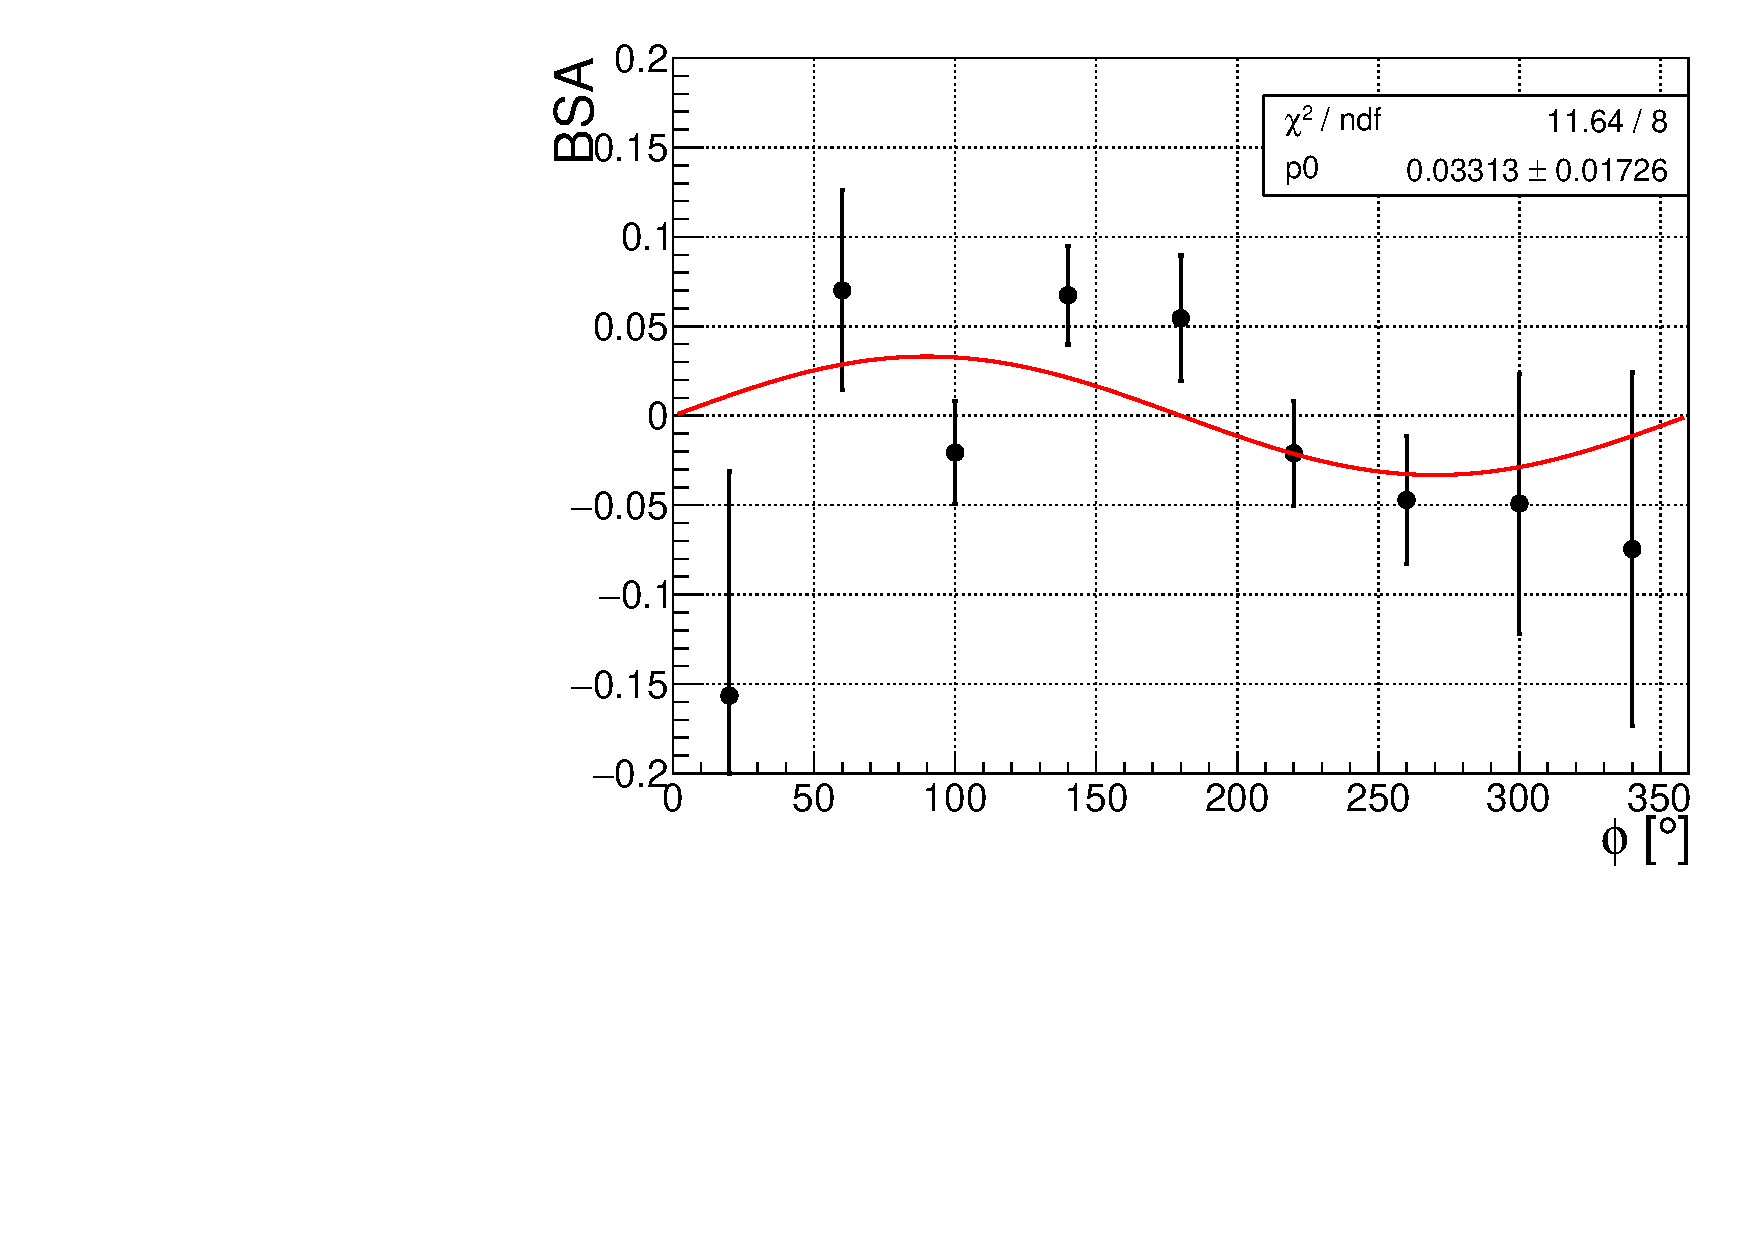
\includegraphics[page=1,width=0.32\linewidth]{figures/eppi0.inb.root.bsa.pdf}
	\includegraphics[page=2,width=0.32\linewidth]{figures/eppi0.inb.root.bsa.pdf}
	\includegraphics[page=3,width=0.32\linewidth]{figures/eppi0.inb.root.bsa.pdf}
	
	\includegraphics[page=5,width=0.32\linewidth]{figures/eppi0.inb.root.bsa.pdf}
	\includegraphics[page=6,width=0.32\linewidth]{figures/eppi0.inb.root.bsa.pdf}
	\includegraphics[page=7,width=0.32\linewidth]{figures/eppi0.inb.root.bsa.pdf}
	
	\includegraphics[page=9,width=0.32\linewidth]{figures/eppi0.inb.root.bsa.pdf}
	\includegraphics[page=10,width=0.32\linewidth]{figures/eppi0.inb.root.bsa.pdf}
	\includegraphics[page=11,width=0.32\linewidth]{figures/eppi0.inb.root.bsa.pdf}
	
	\includegraphics[page=13,width=0.32\linewidth]{figures/eppi0.inb.root.bsa.pdf}
	\includegraphics[page=14,width=0.32\linewidth]{figures/eppi0.inb.root.bsa.pdf}
	\includegraphics[page=15,width=0.32\linewidth]{figures/eppi0.inb.root.bsa.pdf}
	
	\includegraphics[page=17,width=0.32\linewidth]{figures/eppi0.inb.root.bsa.pdf}
	\includegraphics[page=18,width=0.32\linewidth]{figures/eppi0.inb.root.bsa.pdf}
	\includegraphics[page=19,width=0.32\linewidth]{figures/eppi0.inb.root.bsa.pdf}
	
	
	\caption{Beam spin asymmetry as a function of $\phi$ for each of 15 $\{Q^2,x_B,-t\}$ bins for inbending dataset. Each row corresponds to individual $\{Q^2,x_B\}$ bin with 3 $-t$ bins. Fit with $\alpha sin\phi$ function.}
	\label{fig:bsaq2xbtt}
\end{figure}


The relation between beam spin asymmetry and structure functions is following:
\begin{equation}
	BSA = \sqrt{2\epsilon(1-\epsilon)}\frac{\sigma_{LT'}}{\sigma_{0}}
\end{equation}

where $\epsilon$ is beam energy dependent, so to compare results with measurements from other experiments we should extract the ratio of structure functions:
\begin{equation}
	\frac{\sigma_{LT'}}{\sigma_{0}} = \frac{BSA}{\sqrt{2\epsilon(1-\epsilon)}}
\end{equation}

The ratio of structure functions is shown on Fig.~\ref{fig:slts0inq2xb} for each of 5 $\{Q^2,x_B\}$ bins as a function of $-t$.
The BSA measurements from CLAS 6GeV experiments are plotted for comparison for existing low $\{Q^2,x_B\}$ bins.

\begin{figure}[hbt]
	\centering
	\includegraphics[page=4,width=0.32\linewidth]{figures/eppi0.inb.root.bsa.pdf}
	\includegraphics[page=8,width=0.32\linewidth]{figures/eppi0.inb.root.bsa.pdf}
	\includegraphics[page=12,width=0.32\linewidth]{figures/eppi0.inb.root.bsa.pdf}
	
	\includegraphics[page=16,width=0.32\linewidth]{figures/eppi0.inb.root.bsa.pdf}
	\includegraphics[page=20,width=0.32\linewidth]{figures/eppi0.inb.root.bsa.pdf}
	
	
	\caption{$\frac{\sigma_{LT'}}{\sigma_T}$ as a function of $-t$ for 5 $\{Q^2,x_B\}$ bins. Black markers are for the inbending dataset, red markers are for outbending dataset, blue markers are for BSA measurements from CLAS6.}
	\label{fig:slts0inq2xb}
\end{figure}